% ============================================================
%  Rapport DM1 — Vérification du statut ABR pour un arbre binaire
%  L2 Informatique — Algorithmique des Arbres
%  Université Gustave Eiffel
% ============================================================

\documentclass[12pt, a4paper]{article}

% ---------- Encodage & langue ----------
\usepackage[T1]{fontenc}
\usepackage[utf8]{inputenc}
\usepackage[french]{babel}

% ---------- Mise en page ----------
\usepackage[top=2.5cm, bottom=2.5cm, left=2.5cm, right=2.5cm]{geometry}
\usepackage{parskip}          % Espacement entre paragraphes (pas d'indentation)
\usepackage{setspace}
\onehalfspacing               % Interligne 1.5

% ---------- Mathématiques ----------
\usepackage{amsmath}
\usepackage{amssymb}

% ---------- Code source C ----------
\usepackage{listings}
\usepackage{xcolor}

\definecolor{codegreen}{rgb}{0.1,0.5,0.1}
\definecolor{codegray}{rgb}{0.5,0.5,0.5}
\definecolor{codepurple}{rgb}{0.4,0.0,0.6}
\definecolor{backcolour}{rgb}{0.97,0.97,0.97}

\lstdefinestyle{styleC}{
    backgroundcolor=\color{backcolour},
    commentstyle=\color{codegreen}\itshape,
    keywordstyle=\color{codepurple}\bfseries,
    numberstyle=\tiny\color{codegray},
    stringstyle=\color{red},
    basicstyle=\ttfamily\small,
    breakatwhitespace=false,
    breaklines=true,
    captionpos=b,
    keepspaces=true,
    numbers=left,
    numbersep=6pt,
    showspaces=false,
    showstringspaces=false,
    showtabs=false,
    tabsize=2,
    language=C
}
\lstset{style=styleC}

% ---------- Figures & tableaux ----------
\usepackage{graphicx}
\usepackage{float}            % Option [H] pour forcer la position
\usepackage{caption}
\usepackage{subcaption}       % Sous-figures côte à côte
\usepackage{booktabs}         % Tableaux propres (\toprule, \midrule, \bottomrule)
\usepackage{array}

% ---------- Liens cliquables ----------
\usepackage[
    colorlinks=true,
    linkcolor=blue!70!black,
    urlcolor=blue!70!black,
    citecolor=green!50!black
]{hyperref}

% ---------- En-têtes / pieds de page ----------
\usepackage{fancyhdr}
\pagestyle{fancy}
\fancyhf{}
\renewcommand{\headrulewidth}{0.4pt}
\fancyhead[L]{\small DM1 — Vérification du statut ABR}
\fancyhead[R]{\small L2 Informatique — S2}
\fancyfoot[C]{\thepage}

% ---------- Divers ----------
\usepackage{enumitem}         % Personnalisation des listes
\usepackage{tcolorbox}        % Boîtes colorées pour les remarques/résultats clés
\usepackage{titlesec}         % Personnalisation des titres de sections
\usepackage{lipsum}

% Style des titres de section
\titleformat{\section}{\large\bfseries\color{blue!70!black}}{}{0em}{\thesection\quad}
\titleformat{\subsection}{\normalsize\bfseries}{}{0em}{\thesubsection\quad}

% Boîte pour les résultats importants
\tcbuselibrary{skins}
\newtcolorbox{resultatcle}{
    colback=blue!5!white,
    colframe=blue!60!black,
    fonttitle=\bfseries,
    title=Résultat clé
}

% ============================================================
\begin{document}

% ============================================================
%  PAGE DE TITRE
% ============================================================
\begin{titlepage}
    \centering
    \vspace*{1.5cm}

    {\large Université Gustave Eiffel\\[0.3em]
    L2 Informatique — Semestre 2\\[0.3em]
    Algorithmique des Arbres}

    \vspace{2cm}
    \rule{\linewidth}{0.8pt}\\[0.6em]
    {\LARGE\bfseries DM 1 — Vérification du statut \og{}de recherche\fg{}\\[0.4em]
    pour un arbre binaire}\\[0.4em]
    \rule{\linewidth}{0.8pt}

    \vspace{2cm}

    % ---- Membres du binôme / groupe ----
    {\large\bfseries Membres du groupe :}\\[1em]
    \begin{tabular}{ll}
        Raphaël  & \textbf{LIBÉRALE} \\[0.4em]
        Néo & \textbf{RISTIC} \\
        % Ajoute des lignes ici si groupe de 3 ou 4
        % Prénom & \textbf{NOM} \\
        % Prénom & \textbf{NOM} \\
    \end{tabular}

    \vspace{2cm}

    {\large Groupe de TD : \textbf{5}}

    \vfill

    {\large\today}
\end{titlepage}

% ============================================================
%  TABLE DES MATIÈRES
% ============================================================
\tableofcontents
\newpage

% ============================================================
%  PARTIE 1 — RÉALISATION DU DM ET DIFFICULTÉS
% ============================================================
\section{Réalisation du DM et difficultés rencontrées}

% Décrivez brièvement comment vous avez organisé votre travail,
% la répartition des tâches au sein du binôme, et les éventuelles
% difficultés rencontrées lors de l'implémentation.

\subsection{ Réalisation et organisation du travail}

% Exemple de contenu à remplacer :
% Nous avons réparti le travail comme suit : ...
L'organisation du travail a été faite via un dépôt Github, lequel nous a permis de travailler en parallèle sur les différentes tâches du devoir et de synchroniser directement les avancées qu'on faisait. Quant au débuggage, l'outil \texttt{gdb} a été utilisé; Cela a ainsi permis de découvrir des méthodes avancées de débuggage comme l'automatisation des breakpoints et des affichages pour aller plus vite à la source du problème. 

La répartition du travail est la suivante : \linebreak[2]

\begin{table}[H]
	\centering
	\begin{tabular}{>{\bfseries}l p{10cm}}
		\toprule
		\textbf{Membre} & \textbf{Parties traitées} \\
		\midrule
		Raphaël LIBÉRALE
		& \begin{itemize}[noitemsep, topsep=0pt, leftmargin=*]
			\item Section 2.1.1 — Processus de construction des arbres sur un codage générique (\texttt{construit\_quelconque})
			\item Section 2.1.2 — Génération des parcours préfixes des arbres complets, filiformes et quelconques.
			\item Section 2.1.3 — Génération d'arbres ABR et non-ABR complets, filiformes et quelconques
			\item 2.3 Rapport et discussions des résultats
			\end{itemize} \\
		\addlinespace
		Néo RISTIC
		& \begin{itemize}[noitemsep, topsep=0pt, leftmargin=*]
			\item Section 1.1 — Méthode naïve (\texttt{est\_abr\_naif})
			\item Section 1.2 — Méthode optimisée (\texttt{est\_abr\_definition})
			\item Section 1.3 — Méthode infixe (\texttt{est\_abr\_infixe})
			\item Section 2.2 — Protocole expérimental et script Python (\texttt{analyse\_complexite.py})
			\item 2.3 Rapport et discussions des résultats
		  \end{itemize} \\
		\bottomrule
	\end{tabular}
	\caption{Répartition des tâches au sein du binôme.}
	\label{tab:repartition}
\end{table}

\subsection{Difficultés rencontrées}

\paragraph{Raphaël LIBÉRALE :}
% Écris ton ressenti ici
La génération des parcours préfixes depuis les parcours infixes a été technique car il fallait trouver le bon algorithme pour chaque forme d'arbre. Plus particulièrement, hormis le débuggage avec \texttt{gdb} assez long avec chacune des fonctions, la création du parcours préfixe d'un arbre filiforme a pris plusieurs essais d'algorithmes, dont les premiers étaient infructueux. 

 Ensuite, lors des générations d'arbres en fonction des formes, il fallait trouver comment implémenter les caractères de fin pour le codage de l'arbre (en l'occurrence \texttt{-1}); J'ai choisi de le faire avant la création du parcours infixe sur les arbres complets (donc le tableau \texttt{infixe} est de taille $2n + 1$ avant l'appel de la fonction de parcours préfixe, où $n$ est le nombre de nœuds). Pour les arbres filiformes et quelconques, cela se fait lors de la création du parcours infixe (donc \texttt{infixe} est de taille $n$ avant l'appel de la fonction). 
 
 De plus, les tests étant automatisés, j'ai donc dû trouver un substitut des fonctions \texttt{pow}, \texttt{log2} et \texttt{floor} de la bibliothèque \texttt{<math.h>}, car je devais me passer de l'option de compilation \texttt{-lm}. J'ai donc trouvé sur internet une manière de faire en procédant avec les opérations bit à bit implémentées en \texttt{C} afin de reproduire ces calculs


\paragraph{Néo RISTIC :}
% Écris ton ressenti ici
La première difficulté que j'ai rencontré a été la création de la fonction \texttt{est\_abr\_infixe} ou plus particulièrement sa fonction auxiliaire. Cette dernière n'est pas nécessairement longue mais m'a demandé une réelle compréhension récursive de l'algorithme. J'ai donc pris un crayon et une feuille et essayé de comprendre en dessinant des parcours infixe d'arbres binaires.

Mais le plus long a été la partie d'analyse des complexités. Notamment car les résultats graphiques obtenus paraissaient incorrects, ou du moins non représentatifs des complexités théoriques. Au final, nous nous sommes rendu compte que les résultats de notre analyse différaient des résultats théoriques car ils ne représentaient non pas le pire cas mais la moyenne de plusieurs arbres générés aléatoirement. Ainsi les complexités obtenues sont toutes inférieures aux complexités théoriques.

% ============================================================
%  PARTIE 2 — PROTOCOLE EXPÉRIMENTAL
% ============================================================
\section{Protocole expérimental}

Cette section décrit le protocole mis en place pour comparer expérimentalement les trois méthodes de vérification
du statut ABR. L'objectif est qu'un lecteur puisse reproduire intégralement nos expériences.

\subsection{Environnement d'exécution}

% Décris ton environnement : OS, compilateur (clang et version), CPU, RAM, etc.
% Cela est essentiel pour la reproductibilité.

\begin{itemize}
	% Susceptible de changer selon qui est chargé des expériences 
    \item Système d'exploitation : Ubuntu 24.04.4
    \item Compilateur : \texttt{clang}, version 18.1.3
    \item Processeur : Intel(R) Core(TM) Ultra 7 155H
    \item Mémoire vive : 30 Gio de RAM (swap : 8 Gio)
\end{itemize}

\subsection{Types d'arbres générés}

Nous avons généré six types d'arbres binaires sans doublon, résumés dans le tableau ci-dessous.

\begin{table}[H]
    \centering
    \begin{tabular}{lll}
        \toprule
        \textbf{Morphologie} & \textbf{Type} & \textbf{Fonction de génération} \\
        \midrule
        Presque complet & ABR     & \texttt{ABR\_presque\_complet\_alea} \\
        Presque complet & Non-ABR & \texttt{non\_ABR\_presque\_complet\_alea} \\
        Filiforme       & ABR     & \texttt{ABR\_filiforme\_alea} \\
        Filiforme       & Non-ABR & \texttt{non\_ABR\_filiforme\_alea} \\
        Quelconque      & ABR     & \texttt{ABR\_quelconque\_alea} \\
        Quelconque      & Non-ABR & \texttt{non\_ABR\_quelconque\_alea} \\
        \bottomrule
    \end{tabular}
    \caption{Types d'arbres utilisés dans les expériences.}
    \label{tab:types_arbres}
\end{table}

\subsection{Paramètres des mesures}

% Indique les tailles testées, le nombre de répétitions par point de mesure,
% et comment tu as calculé la moyenne.

\begin{itemize}
    \item Tailles testées : $n \in \{100, 600, 1100, \ldots, 9600\}$ noeuds
    \item Nombre de répétitions par point de mesure : $20$
    \item Métrique mesurée : nombre de nœuds visités (type \texttt{long long})
\end{itemize}

\subsection{Format des résultats}

Les résultats sont stockés dans le fichier \texttt{mesures.csv} dont le format de la première ligne est :

\begin{center}
    \texttt{Taille;Morphologie;Methode;Nb\_visites;Temps}
\end{center}

\subsection{Script de compilation et d'exécution}

Grâce à la création d'un \texttt{makefile}, la compilation est hautement simplifiée et cela permet de reproduire les expériences suivantes avec les simples commandes suivantes :

\begin{lstlisting}[language=bash, style=styleC, caption={Compilation et exécution}]
make 
./programme
python3 analyse_complexite.py
\end{lstlisting}

% ============================================================
%  PARTIE 3 — ANALYSE DES RÉSULTATS
% ============================================================
\section{Analyse des résultats}

\subsection{Courbes obtenues}

\begin{figure}[H]
    \centering
    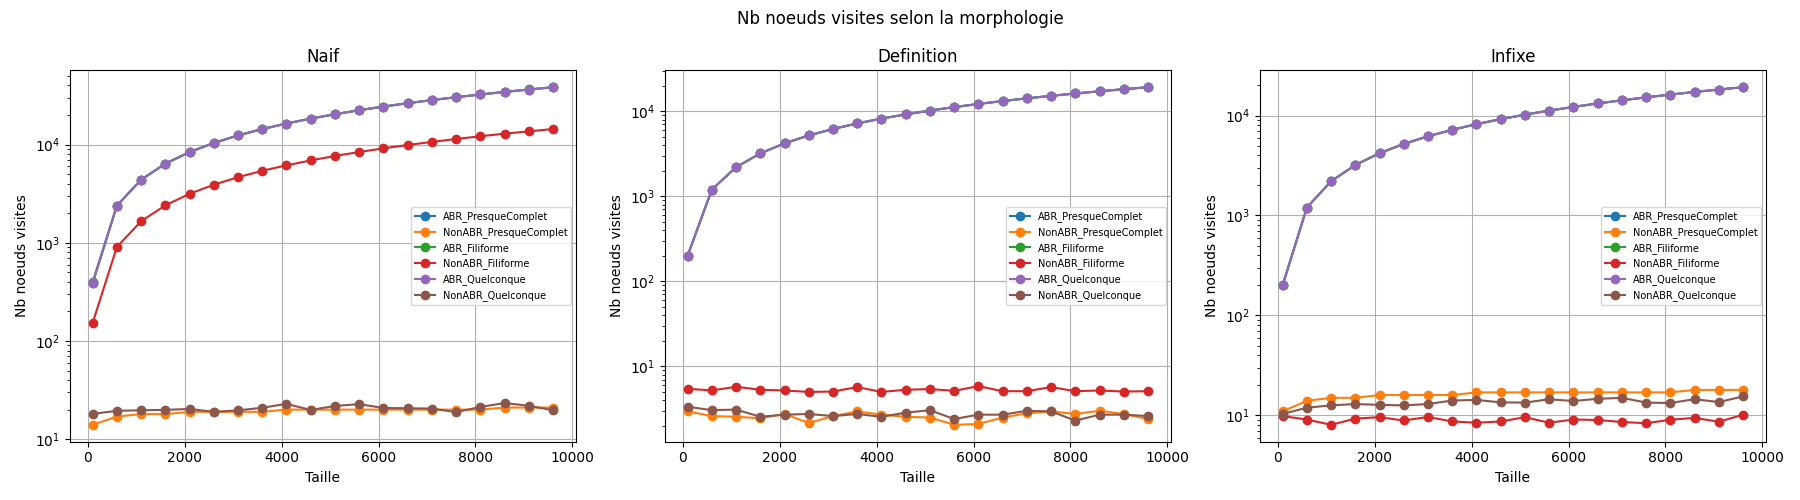
\includegraphics[width=\textwidth]{visites_par_methode.png}
    \caption{Nombre de nœuds visités en fonction de la taille}
    \label{fig:courbe_nb_visites}
\end{figure}

\begin{figure}[H]
    \centering
    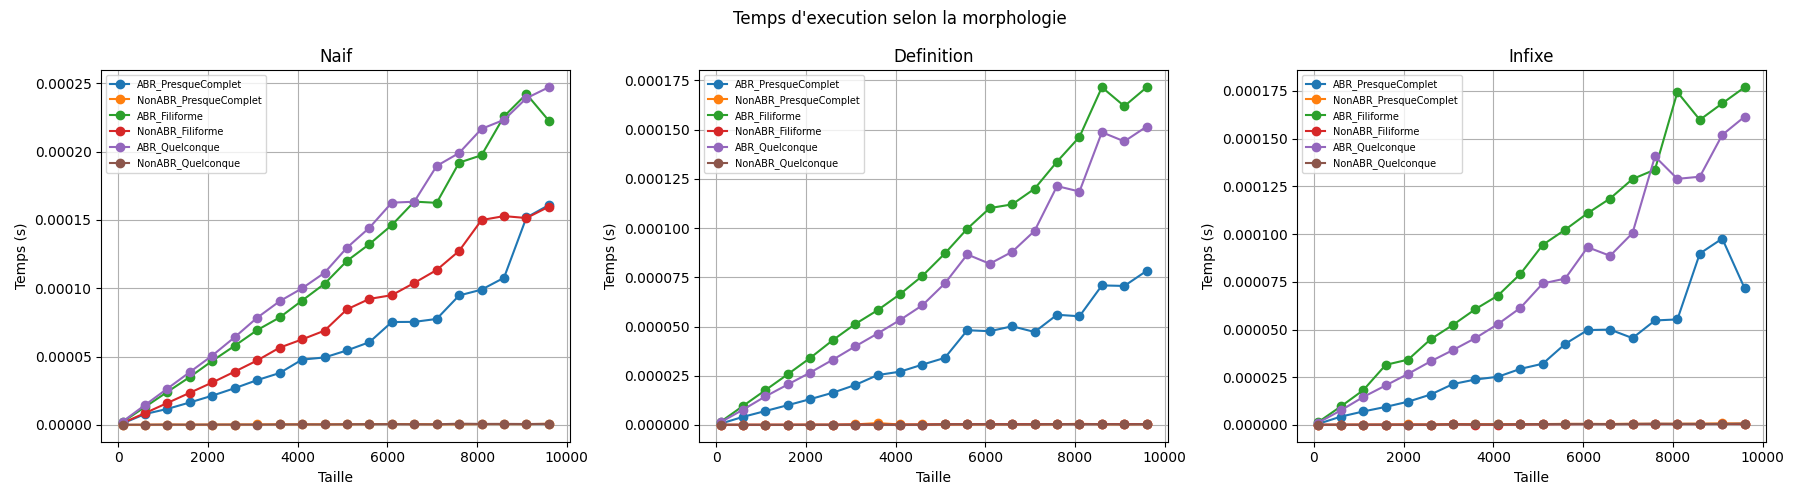
\includegraphics[width=\textwidth]{temps_par_methode.png}
    \caption{Temps en fonction de la taille}
    \label{fig:courbe_temps}
\end{figure}

% ---- 3.2 Complexité théorique et validation expérimentale ----
\subsection{Analyse par méthode}

Nous poserons pour toute cette partie les notations suivantes : 

\begin{itemize}
	\item $h$ : hauteur de l'arbre $\mathit{A}$;
	\item $n$ : nombre de noeuds de l'arbre $\mathit{A}$.
\end{itemize}

\subsubsection{Méthode naïve (\texttt{est\_abr\_naif})}

\paragraph{Complexité théorique.}

Pour chaque nœud, la méthode naïve vérifie récursivement que les sous-arbres gauche et droit
sont eux-mêmes des ABR, puis appelle \texttt{abr\_max} sur le sous-arbre gauche et
\texttt{abr\_min} sur le sous-arbre droit. Ces deux fonctions descendent respectivement
le long de la branche la plus à droite et la plus à gauche du sous-arbre, avec un coût
proportionnel à la hauteur locale $h_{\text{local}}$ du sous-arbre considéré.
En sommant sur tous les nœuds, la complexité dans le pire cas est $\mathcal{O}(n \cdot h)$,
où $h$ est la hauteur de l'arbre. Dans le pire cas absolu (arbre filiforme), $h = n - 1$,
ce qui donne une complexité en $\mathcal{O}(n^2)$.

\begin{resultatcle}
	Complexité temporelle de \texttt{est\_abr\_naif} : $\mathcal{O}(n^2)$ dans le pire cas.
\end{resultatcle}

\paragraph{Validation expérimentale.}

Le pire cas théorique $\mathcal{O}(n^2)$ est atteint sur un arbre filiforme dont tous les
nœuds n'ont que des fils gauches (ou que des fils droits), car \texttt{abr\_max} doit alors
descendre une chaîne de longueur $k$ au niveau $k$, et on doit faire ceci $n$ fois. En effet, on va d'abord visiter $h$ nœuds, puis $h-1$, puis $h-2$, $\ldots$, puis $1$, ce qui donne la somme $$\sum_{k=1}^{n} k = \frac{n(n+1)}{2}$$ qui est bien quadratique. 

\begin{figure}[H]
	\centering
	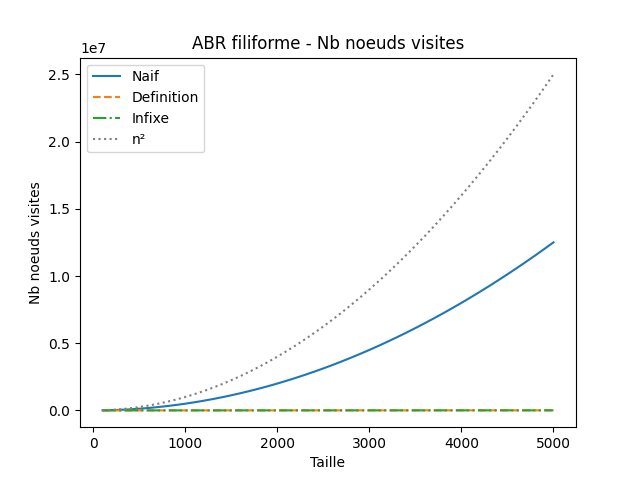
\includegraphics[width=0.75\textwidth]{filiforme_pire_cas_visites.png}
	\caption{Graphique du nombre de nœuds visités pour un filiforme de pire cas avec tous les enfants dans une seule direction.}
	\label{fig:courbe_abr}
\end{figure}

Cependant, un tel arbre filiforme entièrement orienté dans un seul sens
a une probabilité de $\frac{1}{2^{n-1}}$ d'être généré aléatoirement, soit $\frac{1}{2^{999}}
\approx 0$ pour $n = 1000$. En pratique, un arbre filiforme aléatoire alterne les directions
gauche et droite, de sorte que \texttt{abr\_max} et \texttt{abr\_min} coûtent $\mathcal{O}(1)$
en moyenne à chaque appel : la branche latérale opposée est quasi-inexistante.

Le nombre total de visites s'écrit alors :
\[
T(n) = \underbrace{2n + 1}_{\text{parcours récursif principal}} +
\underbrace{2n}_{\text{appels à \texttt{abr\_max} et \texttt{abr\_min}, coût amorti } \mathcal{O}(1)}
= 4n + 1
\]
ce qui est bien linéaire, conformément à ce qu'on observe sur les courbes
(pente constante $\approx 4$ en échelle linéaire).

Pour un arbre presque complet, la hauteur vaut $h = \lfloor \log_2(n) \rfloor$.
Pour un nœud situé à la profondeur d, son sous-arbre gauche a une hauteur de $h - d$. 
L'appel à $\texttt{abr\_max}$ sur ce sous-arbre doit descendre le long de la branche la plus à droite, ce qui coûte exactement $h - d$ visites.
On peut donc calculer :
\[
\sum_{d=0}^{h} 2^d \cdot (h - d) = 2^h \sum_{k=0}^{h} \frac{k}{2^k} \approx 2n \cdot 2 = 4n
\]
car la série $\sum_{k=0}^{\infty} \frac{k}{2^k}$ converge vers $2$.
La complexité réelle est donc également $\Theta(n)$, bien que la borne
théorique $\mathcal{O}(n \log n)$ soit formellement correcte mais très pessimiste.

\paragraph{Différences selon la morphologie.}

En pratique, les trois morphologies ABR (presque complet, filiforme, quelconque)
produisent toutes une courbe de visites en $\approx 4n$, sans différence notable.
Cela confirme que la constante multiplicative devant $n$ est insensible à la forme
de l'arbre, dès lors que les branches latérales restent courtes en moyenne.

La différence apparaît en revanche sur les \emph{temps d'exécution} :
\texttt{ABR\_Filiforme} est nettement plus lent que \texttt{ABR\_PresqueComplet}
à nombre de visites égal, en raison de la profondeur de récursion $h = n$ qui
génère $n$ frames de pile consécutives et davantage de défauts de cache mémoire.

Pour les non-ABR, le comportement diverge fortement selon la morphologie.
\texttt{NonABR\_Filiforme} reste linéaire ($\approx 1.5n$ visites) car la violation
est placée à une position aléatoire dans la chaîne~: il faut en moyenne parcourir
la moitié de l'arbre avant de la détecter. En revanche, \texttt{NonABR\_PresqueComplet}
et \texttt{NonABR\_Quelconque} sont quasi-constants, la violation étant statistiquement
proche de la racine dans notre méthode de génération.


% ---- Méthode optimisée ----
\subsubsection{Méthode optimisée (\texttt{est\_abr\_definition})}

\paragraph{Complexité théorique.}

La méthode optimisée propage des bornes $[\min, \max]$ à travers les appels récursifs,
visitant chaque nœud exactement une fois (nœuds réels et sentinelles NULL incluses).
Il n'y a aucun reparcours de sous-arbre. Sa complexité est donc $\mathcal{O}(n)$
dans tous les cas, avec une constante très proche de $2$ ($n$ nœuds réels +
$n+1$ appels sur NULL).

\begin{resultatcle}
	Complexité temporelle de \texttt{est\_abr\_definition} : $\mathcal{O}(n)$ dans le pire cas.
\end{resultatcle}

\paragraph{Validation expérimentale.}

Les courbes montrent $2n + 1$ visites pour tous les ABR, quelle que soit la morphologie (les courbes sont superposées car la différences de quelques centaines de noeuds est trop faible pour être visible sur le graphique), 
ce qui correspond exactement au nombre de nœuds réels plus le nombre de feuilles \texttt{NULL}
dans un arbre binaire à $n$ nœuds. Cette valeur est indépendante de la forme de l'arbre,
ce qui est validé par la superposition des courbes \texttt{ABR\_PresqueComplet} et
\texttt{ABR\_Filiforme} en échelle logarithmique.

Pour les non-ABR, la détection est quasi-immédiate ($\mathcal{O}(1)$) dès que la
violation est proche de la racine : la borne propagée est violée au premier nœud
concerné et la récursion s'interrompt. Cela se traduit par des courbes plates
au voisinage de $2$ et $8$ visites pour les trois morphologies.
\paragraph{Différences selon la morphologie.}

Pour les ABR, il n'y a aucune différence entre les morphologies : le nombre de
visites est strictement $2n+1$ dans tous les cas. Pour les non-ABR, la différence
dépend uniquement de la \emph{position de la première violation} dans l'ordre de
parcours préfixe, qui est déterminée par la méthode de génération et non par la
forme de l'arbre.


% ---- Méthode infixe ----
\subsubsection{Méthode par parcours infixe (\texttt{est\_abr\_infixe})}

\paragraph{Complexité théorique.}

La méthode infixe réalise un parcours infixe de l'arbre en s'interrompant dès la
première violation de l'ordre croissant. Dans le meilleur cas (violation au premier
nœud visité en ordre infixe, c'est-à-dire au nœud le plus à gauche), sa complexité
est $\mathcal{O}(h)$, où $h$ est la hauteur de l'arbre, car il faut descendre jusqu'au
premier nœud infixe avant de détecter l'anomalie. Dans le pire cas (arbre ABR),
le parcours est intégralement réalisé et la complexité est $\mathcal{O}(n)$.

\begin{resultatcle}
	Complexité temporelle de \texttt{est\_abr\_infixe} : $\mathcal{O}(n)$ dans le pire cas.
\end{resultatcle}

\paragraph{Validation expérimentale.}

Les courbes de visites pour les ABR sont superposées à celles de la méthode "Définition"
($2n+1$ visites), ce qui confirme que le parcours infixe complet visite exactement
autant de nœuds. Pour les non-ABR, les courbes sont quasi-constantes mais légèrement
supérieures à celles de la méthode "Définition" : en effet, la méthode infixe doit
d'abord descendre jusqu'au nœud le plus à gauche ($\mathcal{O}(h)$ visites) avant
de commencer à comparer, alors que la méthode Définition peut détecter une violation
dès la racine.

\paragraph{Différences selon la morphologie.}

Pour les ABR, le constat est identique à la méthode "Définition" : $2n+1$ visites
quelle que soit la morphologie. Pour les non-ABR sur arbre filiforme, le comportement
est quasi-constant ($\approx 9$ à $10$ visites observées) car la violation de l'ordre
croissant est détectée très tôt dans le parcours infixe indépendamment de la position
de la violation dans l'arbre.


% ---- Comparaison des méthodes ----
\subsection{Comparaison des trois méthodes}

\subsubsection{Cas des arbres qui sont des ABR}

Sur les ABR, les trois méthodes visitent toutes $\Theta(n)$ nœuds, mais avec des
constantes différentes. La méthode naïve visite environ $4n$ nœuds, contre $2n+1$
pour les méthodes "Définition" et "Infixe". L'écart de constante (facteur $\approx 2$) se retrouve directement sur les temps d'exécution. Les méthodes "Définition" et "Infixe" sont donc systématiquement plus efficaces sur les ABR, avec une performance
quasi-identique entre elles.

\subsubsection{Cas des arbres qui ne sont pas des ABR}

L'interruption anticipée est le facteur déterminant. La méthode Définition est la
plus efficace : elle peut détecter une violation dès la racine en $\mathcal{O}(1)$,
car la borne $[\min, \max]$ est vérifiée avant toute récursion. La méthode Infixe
doit d'abord descendre jusqu'au nœud le plus à gauche avant de commencer les
comparaisons, ce qui lui coûte $\mathcal{O}(h)$ visites même si la violation se
trouve proche de la racine — d'où les $\approx 9$ à $10$ visites observées.

La méthode naïve est la plus pénalisée sur les non-ABR filiformes : elle récurse
d'abord jusqu'aux feuilles pour valider les sous-arbres, puis remonte pour comparer,
de sorte qu'elle doit parcourir en moyenne la moitié de l'arbre avant de détecter
la violation, soit $\approx 1.5n$ visites.

\subsubsection{Synthèse}

\begin{table}[H]
	\centering
	\setlength{\tabcolsep}{5pt}
	\begin{tabular}{l p{3.2cm} p{3.2cm} p{3.2cm}}
		\toprule
		& \textbf{Naïve} & \textbf{Optimisée} & \textbf{Infixe} \\
		\midrule
		Complexité pire cas
		& $\mathcal{O}(n^2)$
		& $\mathcal{O}(n)$
		& $\mathcal{O}(n)$ \\
		Complexité pratique ABR
		& $\Theta(4n)$
		& $\Theta(2n)$
		& $\Theta(2n)$ \\
		Complexité meilleur cas
		& $\mathcal{O}(1)$
		& $\mathcal{O}(1)$
		& $\mathcal{O}(h)$ \\
		Avantage principal
		& Simple à implémenter
		& Optimale en tous cas
		& Découle naturellement de la propriété infixe \\
		Inconvénient principal
		& Constante $\times 2$ sur les ABR
		& Moins intuitive à concevoir
		& Meilleur cas en $\mathcal{O}(h)$ \\
		\bottomrule
	\end{tabular}
	\caption{Synthèse comparative des trois méthodes.}
	\label{tab:synthese}
\end{table}

En conclusion, la méthode "Définition" est à recommander dans tous les cas : elle
est optimale en $\mathcal{O}(n)$ sur les ABR, détecte les violations en $\mathcal{O}(1)$
dès la racine sur les non-ABR, et sa constante multiplicative ($\approx 2$) est
la plus faible des trois. La méthode "Infixe" lui est équivalente sur les ABR mais
légèrement moins efficace sur les non-ABR. La méthode naïve, bien que correcte,
est à éviter en pratique en raison de son coût double sur les ABR et de sa
sensibilité aux arbres filiformes.
% ============================================================
%  CONCLUSION
% ============================================================
\section*{Conclusion}
\addcontentsline{toc}{section}{Conclusion}

Ce devoir nous a permis d'implémenter et de comparer trois méthodes de vérification
du statut ABR, en confrontant leur complexité théorique à des mesures expérimentales.

On voit en particulier que les complexités théoriques sont en pratiques très différentes 
des complexités pratiques .

La méthode "Définition" s'impose finalement comme la plus efficace dans tous les cas :
complexité $\mathcal{O}(n)$ garantie, détection en $\mathcal{O}(1)$ dès la racine
pour les non-ABR, et constante multiplicative la plus faible. Ce DM illustre ainsi
qu'une analyse algorithmique associée à une validation expérimentale
est indispensable pour choisir la bonne implémentation en pratique.

\end{document}

